\documentclass{beamer}

\usepackage{graphicx, color}
\usepackage{alltt}
\usepackage{booktabs, calc, rotating}
\usepackage[round]{natbib}
\usepackage{pdfpages, subfigure}
\usepackage{multicol}
\usepackage{amsmath, amsbsy, amssymb, amsthm, graphicx}
\usepackage[english]{babel}
\usepackage{xkeyval} 
\usepackage{xfrac}
\usepackage[normalem]{ulem}
 \usepackage{multirow, fancyvrb} 
\usepackage{tikz, geometry, tkz-graph, xcolor}

\graphicspath{{figure/}}

\usetikzlibrary{arrows,positioning} 
\tikzset{
    %Define standard arrow tip
    >=stealth',
    %Define style for boxes
    punkt/.style={
           rectangle,
           rounded corners,
           draw=black, very thick,
           text width=6.5em,
           minimum height=2em,
           text centered},
    % Define arrow style
    pil/.style={
           ->,
           thick,
           shorten <=2pt,
           shorten >=2pt,}
}


\newcommand{\cov}{\mathrm{cov}}
\newcommand{\dif}{\mathrm{d}}
\newcommand{\bigbrk}{\vspace*{2in}}
\newcommand{\smallbrk}{\vspace*{.1in}}
\newcommand{\midbrk}{\vspace*{1in}}
\newcommand{\red}[1]{{\color{red}#1}}
\newcommand{\blue}[1]{{\color{blue}#1}}
\newcommand{\green}[1]{{\color{green}#1}}
\newcommand{\calc}[1]{{\fbox{\mbox{#1}}}}
\newcommand{\Var}{\mathrm{Var}}%
\newcommand{\Cov}{\mathrm{Cov}}%

\mode<presentation>
{
  \usetheme{UTD}
  \usecolortheme[RGB={200,0,0}]{structure}
  \setbeamercovered{transparent}
}

\usepackage[latin1]{inputenc}
\usepackage{times}
\usepackage[T1]{fontenc}

\fvset{frame=single,framesep=1mm,fontfamily=courier,fontsize=\scriptsize,numbers=left,framerule=.3mm,numbersep=1mm,commandchars=\\\{\}}


\title[STAT 5353.001]{STAT 5353: Probability and Statistics for Data Science and Bioinformatics}
%\small{Textbook coverage: Chapter 1: Introduction}}
\author[Steven Chiou]{Steven Chiou}
\institute[UTD]{Department of Mathematical Sciences, \\ University of Texas at Dallas}
\date{}

\begin{document}

\begin{frame}
  \titlepage
\end{frame}

\setbeamercolor*{item}{fg=red}
\bgroup
\usebackgroundtemplate{%
\tikz[overlay,remember picture] \node[opacity=0.05, at=(current page.center)] {
   
\includegraphics[height=\paperheight,width=\paperwidth]{UTDbg}};}


%\section[Outline]{}
%\begin{frame}
%\frametitle{Outline}
%  \tableofcontents
%\end{frame}


\section{Syllabus overview}
\begin{frame}
\frametitle{Course information}
\begin{center}
%\renewcommand{\arraystretch}{1.2}
\begin{tabular}{p{.25\textwidth} p{.75\textwidth}}
Instructor & Sy Han (Steven) Chiou\\
Email address & schiou@utdallas.edu\\
Office Location & FO 2.410A\\
Office Hours & Tuesday, Thursday, 12:30 pm - 1:30 pm, \\
&or by appointment.
\end{tabular}
\end{center}
\end{frame}

\begin{frame}
\frametitle{Required text}
\begin{columns}
    \column{0.5\textwidth}
\begin{center}
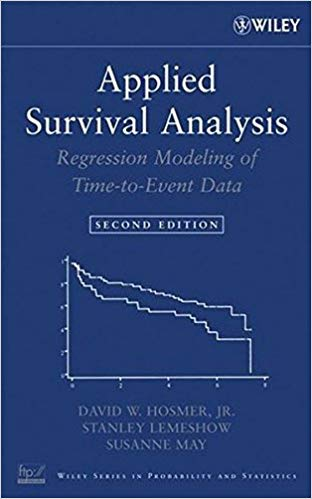
\includegraphics[scale = .4]{coursebook}
\end{center}
    \column{0.5\textwidth}
\begin{itemize}
\item David W. Hosmer, Stanley Lemeshow, and Susanne May
\item 2nd edition
\item ISBN: 978-0-471-75499-2
\end{itemize}
\end{columns}
\end{frame}

\begin{frame}
\frametitle{Prerequisite}
\begin{itemize}
\item Calculus through multivariate calculus 
\item Basic knowledge of regression methods
\item Statistical methods for estimation and inferences
\item Basic knowledge about \texttt{R} 
\item Basic knowledge about \texttt{GitHub} 
\end{itemize}
\end{frame}

\begin{frame}
\frametitle{Course website}
\begin{itemize}
\item \url{http://elearning.utdallas.edu/}
\item The website will contain 
\begin{itemize}
\item Syllabus
\item Lecture notes, both the original and annotated versions
\item \texttt{R} scripts
\item Homework and exams
\end{itemize}
\end{itemize}
\end{frame}

\begin{frame}
\frametitle{Grading criteria}
\begin{itemize}
\item Homework (50\%)
\begin{itemize}
\item Biweekly; maybe 5 $\sim$ 6 assignments
\item Requires \texttt{R}
\item Be prepared using \textit{markdown} or \textit{knitr}
\item Due in class or submit via \texttt{GitHub}.
\end{itemize}
\item 1 midterm \& 1 Final (25\% each)
\begin{itemize}
\item Take-home portion that requires \texttt{R}
\item One week to complete.
\end{itemize}
\item Grade assignment:\\\vspace{.5cm}
\centering
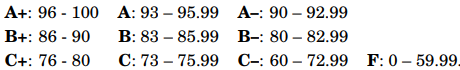
\includegraphics[scale = .4]{grade}
\end{itemize}
\end{frame}

\begin{frame}
\frametitle{Tentative course schedule}
\centering\vspace{-.2cm}
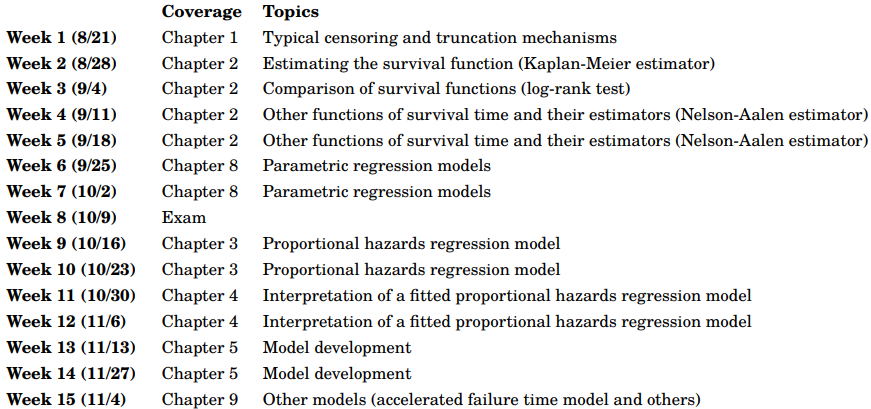
\includegraphics[scale = .4]{schedule}
\end{frame}

\end{document}

